\chapter{Коллективная азимутальная анизотропия в столкновениях тяжелых ионов} \label{chapt1}

\section{Центральность столкновения}

В результате столкновения тяжелых ионов, в области перекрытия образуется сильно взаимодействующая материя, свойства которой сильно зависят от размера сталкивающихся ядер, и от энергии столкновения.
При столкновении тяжелых ядер, при энергиях в несколько ГэВ на нуклон налетающего ядра, время пролёта ионов сравнимо со временем существования материи в области перекрытия.
Процесс столкновения двух ядер можно условно разделить на несколько этапов.

Начальная фаза определяет геометрию столкновения, а именно прицельный параметр $b$ --- расстояние между центрами сталкивающихся ядер, пространственное распределение нуклонов, число нуклонов-партисипантов, испытывающих в ходе столкновения неупругие рассеяния и число нуклонов-спектаторов, взаимодействующих лишь упруго.  
Экспериментальное измерение прицельного параметра невозможно, поэтому необходима физическая наблюдаемая, по которой можно судить о геометрии столкновения.
Этой наблюдаемой является центральность столкновения, как группа событий относящихся к данной части полного неупругого сечения взаимодействия:
%
\begin{equation}
    C_S = \frac{1}{ \sigma_{inel}^{AA} } \int_{S_1}^{S_2} \frac{d\sigma}{dS}dS,
\end{equation}
где $C_S$ --- центральность столкновения по выбранному эстиматору центральности, $\sigma_{inel}^{AA}$ --- полное сечение неупругого взаимодействия двух ядер, $S_{1,2}$ --- границы класса центральности.
В качестве эстиматора класса центральности в эксперименте часто выбирается множественность частиц, либо величина пропорциональная ей.
При помощи метода Монте-Карло Глаубера разыгрываются геометрические параметры столкновения, такие как прицельный параметр $b$, число партисипантов $N_{part}$, число бинарных неупругих рассеяний $N_{col}$.
Используя отрицательное биномиальное распределение и выход Монте-Карло Глаубера моделирования подбирается множественность рожденых частиц, которая будет аппроксимировать эксеприментальное распределение множественности.
На основании этого затем определяются классы центральности и извлекаются средние значения геометрических параметров для каждого класса.

\section{Коллективные эффекты в столкновениях тяжелых ядер}

При скоростях налетающего ядра, превышающих скорость звука в ядерной материи при при обычных условиях ($\beta_S=0.2$)~\cite{Weber:1998aa}, нуклоны не могут покинуть область перекрытия достаточно быстро, и образуется зона высокой плотности.
В зависимости от уравнения состояния, которое связывает давление с плотностью и температурой, материя в зоне перекрытия может достигать условий, которые описываются средней плотностью и температурой.
В этих условиях могут быть созданы новые частицы, а их число и характер эмиссии могут быть использованы для исследования глобальных свойств вещества.
Отклонение плотным веществом в области перекрытия, остатков налетающего ядра с положительной быстротой происходит в направлении $+x$, что приводит к $\langle p_x \rangle  > 0$, а остатки ядра с отрицательной быстротой отклоняются в направлении -x, таким образом, имея $\langle p_x \rangle < 0$.
Таким образом, направленный поток остатков налетающего ядра является положительным для частиц с положительной бысротой и отрицательным для частиц с отрицательной быстротой.
Измерения направленного потока частиц, относительно плоскости симметрии определенной спектаторами даёт информацию о времени взаимодействия рожденных частиц с областью перекрытия.
Положительный направленный поток частиц относительно плоскости симметрии остатков налетающего ядра говорит о довольно большом времени взаимодействия, при котором материя в области перекрытия успевает смешаться с холодной спектаторной материей.
Эллиптический поток $v_2$ несёт информацию о давлении в области перектия сталкивающихся ионов.
При энергиях порядка 1~ГэВ, значения $v_2$ отрицательные относительно плоскости симметрии спектаторов.
Остатки сталкивающихся ядер блокируют вылет частиц в плоскости реакции, что определяет вылет частиц перпендикулярно плоскости реакции.
Чем выше давление, достигаемое в области перекрытия, тем выше будут значения $v_2$.
Схематически эти механизмы изображены на рис.~\ref{fig:bounce_off}.
%
\begin{figure}[ht]
\begin{center}
    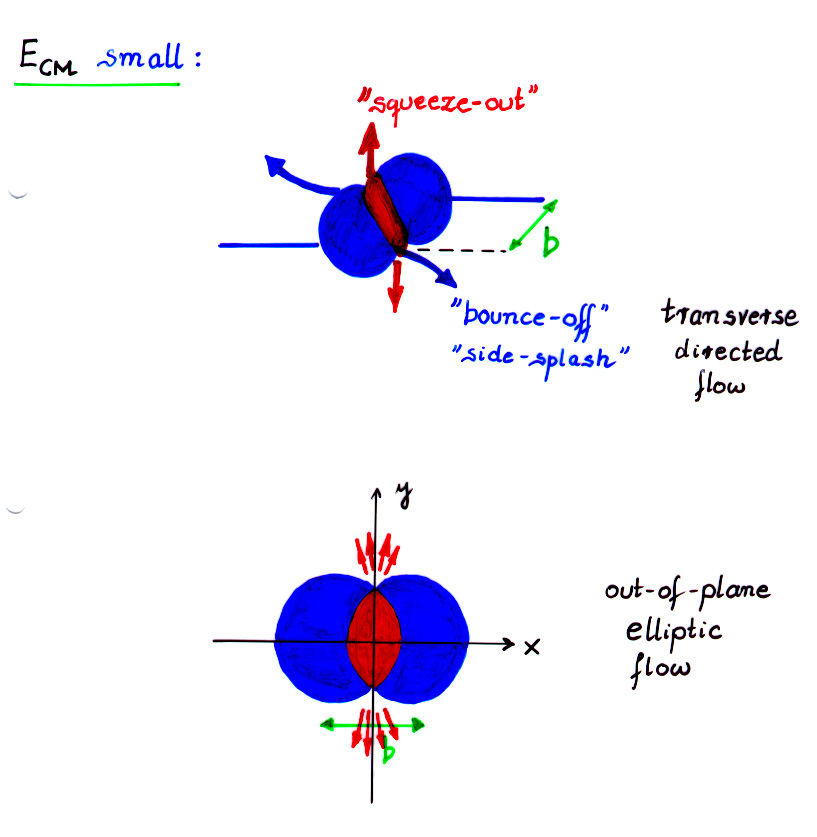
\includegraphics[width=0.75\linewidth]{images/bounce_off.jpg}
    \caption{Схематичное изображение механизмов рождения направленного (bounce-off) эллиптического (squeeze-out) потоков.}
    \label{fig:bounce_off}
\end{center}
\end{figure}
%

Партисипанты, или нуклоны сталкиващихся ядре претерпевают многократные рассеяния.
В результате рождаются новые частицы и изменяются импульсы частиц, составляющих материю в области перекрытия.
Если время взаимодействия достаточно велико, то материю в области перекрытия можно описать при помощи статистических величин: средняя плотность, средняя температура и т.д..
При многократном рассеянии частиц, составляющих материю в области перекрытия, может происходить подпороговое рождение частиц.
Сравнивая коллективные потоки различных типов частиц, рожденных в области перекрытия можно судить о степени термализации или релаксации энергии в области перекрытия.
Чем ближе потоки различных типов сталкивающихся частиц к среднему значению, тем больше степень термализации материи.
По степени термализации можно судить о времени существования материии в области перекрытия.  

Реакция и развитие коллективных эффектов останавливаются на стадии столкновения, обычно называемой фриз-аут. 
В этой фазе плотности достаточно малы, чтобы в течение типичной длины пролета больше не происходило взаимодействия.
Хотя многие наблюдаемые (например, спектры рожденных частиц) теряют память о начальных условиях во время процесса эволюции, ожидается, что коллективные потоки адронов несут информацию о самых ранних этапах эволюции~\cite{Herrmann:1999wu}.
Коллективные потоки рожденных в столкновении адронов сильно зависят от начальной геометрии столкновения.
Коллективное движение рожденых адронов обусловлено взаимодействием частиц составляющих материю в области перекрытия.
Характер этого взаимодействия обусловлен свойствами материи, которые описываются уравнением состояния.
Поэтому зная изначальную геометрию столкновения, которая определяется центральностью и измеряя итоговую анизотропию рожденных частиц можно извлечь уравнение состояния сильновзаимодействующей материи.

Коллективное движение частиц приводит к корреляции импульсов рожденных адронов.
Таким образом, изучая эту корреляцию, можно колличественно оценить коллективные эффекты.
Однако это не единственный канал, по которому импульсы рожденных частиц могут быть скоррелированы.
К примеру, импульсы частиц, рожденных в слабом или сильном распаде резонанса относятся следующим образом:
%
\begin{equation}
    P = P_1 + P_2,
\end{equation}
где $P$ --- 4-импульс резонанса, $P_{1,2}$ --- импульсы рожденных в распаде частиц.
Также в силу сохранения поперечного (полного) импульса системы справедливо следующее соотношение:
%
\begin{equation}
    \sum_{k=1}^{N} \vec{p_T}^k = 0,
\end{equation}
где $N$ --- множественность рожденных частиц, $\vec{p_{T}}^k$ --- поперечный импульс $k$-й частицы.
Корреляция импульсов частиц, рожденной в бинарном столкновении частиц, составляющих материю тоже подчиняется законам сохранения импульса:
%
\begin{equation}
    P_1 + P_2 = P_3 + P_4 + P_5.
\end{equation}

Описанные выше эффекты не имеют отношения к коллективному движению частиц, однако обеспечивают корреляцию импульсов.
Такие эффекты носят название непотоковых корреляций и осложняют измерение коллективных эффектов.
Поэтому для подавления непотоковых эффектов чаще всего рассматривается корреляция большого колличества частиц.
Также для подавления корреляций не связанных с коллективным движением частиц можно рассматривать корреляцию областей со значительнми разделением по кинематике.
Оценка вклада остаточных непотоковых корреляций является важной задачей при измерении коллективных эффектов.

\section{Основыне определения}

Методы измерения коллективных потоков довольно просто описать в терминах векторов.
Для измерения азимутальных потоков каждой частице ставится в соответствие единичный вектор $u_1$ в плоскости поперечной плоскости пучка на основании импульса частицы:
%
\begin{equation}
    \vec{u_1} = (x_1, y_1) = \frac{\vec{p_T}}{p_T} = ( \cos \varphi, \sin \varphi ),
\end{equation}
%
где $\varphi$ --- азимутальный угол частицы. 
При очень большом количестве частиц в одном событии ($N \gg 1$), сумму по всем частицам можно переписать в виде интеграла:
%
\begin{equation}
    \langle \vec{u_1} \rangle = \sum_{k=1}^{N} u_1 = \int_{-\pi}^{\pi} \vec{u_1} \rho(\phi-\Psi_{R}) d\phi
\end{equation}
Рассмотрим интеграл по $x$-компоненте $u_1$ вектора:
%
\begin{equation}
    \int_{-\pi}^{\pi} x_1 \rho(\phi-\Psi_{R}) d\phi =
    \int_{-\pi}^{\pi} \cos( \phi - \Psi_{R} + \Psi_{R} ) \rho(\phi - \Psi_R) = V_1 \cos(\Psi_R), 
\end{equation}
где $V_1$ пропорционален множественности частиц $N$ и значению $v_1$ для данной группы частиц в данном событии.
Аналогичные преобразования можно выполнить и для $y$-компоненты $u_1$-вектора, получив $V_1\sin(\Psi_R)$.
Таким образом, суммируя по группе $u_1$-векторов одном событии можно получить оценку угла плоскости реакции $\Psi_R$ в данном событии.

Эта оцнека, определяемая суммой единичных векторов частиц носит название $Q_1$-вектора:
%
\begin{equation}
    \vec{Q_1} = \frac{1}{C} \sum_{k=1}^{N} w_k u_1^k = \frac{|Q_1|}{C} (\cos{\Psi}, \sin{\Psi}) ,
\end{equation}
%
где $k$ --- индекс частицы в группе, $w_k$ --- вес $k$-го вектора, $N$ --- множественность частиц в группе, $\Psi$ --- угол плоскости симметрии данного события, $|Q_1|$ --- модуь $Q_1$-вектора и $C$ --- нормировочный коэффициент. 
Чем больше число частиц в событии, тем ближе оценка угла плоскости симметрии к реальной ориентации плоскости реакции.
%
\begin{equation}
    \lim_{N \xrightarrow{} \infty} \frac{1}{C} \sum_{k=1}^{N} w_k u_1^k = \frac{|Q_1|}{C} (\cos{\Psi_R}}, \sin{\Psi_R}) ,
\end{equation}

\section{Методы плоскости события и скалярного произведеления}

Выбор значения нормировочного коэффициента определяет метод измерения направленного потока. 
В работе рассмотрены два метода: плоскости события (EP) и скалярного произведения (SP). 

Метод плоскости события (EP) требует такую нормировку, что модуль каждого $Q_1$-вектора был равен 1, что соответствует $C=|Q_1|$. 
В работах~\cite{Borghini:2001vi, Bhalerao:2006tp} было показано, что в таком случае, измеренное значение потока $v_1^\{EP\}$ нелинейно зависит от множественности частиц, использованных для вычисления $Q_n$-вектора, а также от значения самого потока. 
В пределе большого количества частиц и большого значения потока ($v_1 \sqrt{M} \gg 1$), измеренные значения стремятся к среднему значению $v_1$: $v_1\{EP\} \xrightarrow{} \langle v_1 \rangle$. 
В случае малого числа частиц, использованных для построения $Q_1$-вектора, а также малых значениях потока ($v_1 \sqrt{M} \ll 1$), измерения стремятся к корню среднего квадрата $ v_1\{EP\} \xrightarrow{} \sqrt{ \langle v_1^2 \rangle }$.
Таким образом, экспериментально измеренные значения $v_1\{EP\}$ находятся между двумя пределами: $ \langle v_1 \rangle \leq v_1\{EP\} \leq \sqrt{ \langle v_1^2 \rangle } $.
В зависимости от реального значения $v_1$ (который определяется энергией столкновения и размером сталкивающихся ядер) и множественности частиц (которая зависит от энергии, размера ядер и аксептанса установки), измеренные значения $v_1\{EP\}$ могут лежать ближе к правому или левому пределам.

Второй метод, скалярного произведения (SP), требует нормировку на сумму весов $C=\sum_{k=1}^N w_k$.
Таким образом, модуль $Q_1$-вектора сохраняет информацию о множественности частиц, использованных для его построения, а также их $v_1$: $|Q_1| \propto v_1 M$.
Использование такой нормировки дает значения $v_1\{SP\} \xrightarrow{} \sqrt{\langle v_1^2 \rangle}$ независимо от измеренной множественности частиц, а также их $v_1$.

\section{Разрешение плоскости симметрии}

Экспериментально направленный поток можно определить как проекцию $u_1$-вектора частиц на плоскость симметрии события:
%
\begin{equation}
    v_1' =  \langle u_1 Q_1 \rangle = 
    V_1 \langle \cos\phi \cos \Psi \rangle + V_1 \langle \sin\phi \sin\Psi \rangle,
\end{equation}
%
где диагональные члены равны нулю в силу симметрии столкновения, а коэффициент $V_1$ появляется в силу усреднения модулей вектора $Q_1$.
Раскрывая тригонометрические выражения в угловых скобках, можно получить:
%
\begin{equation}
    \langle \cos\phi \cos \Psi \rangle = \langle \cos( \phi - \Psi ) \rangle = 
    \langle \cos( \phi - \Psi + \Psi_R - \Psi_R ) \rangle =
    \langle \cos( \phi - \Psi_R ) \cos(\Psi - \Psi_R ) \rangle
\end{equation}
%
Аналогичные преобразования можно выполнить и для синусов. 
Таким образом, измеренные значения направленного потока имеют вид:
%
\begin{equation}
    v_1' =  \langle u_1 Q_1 \rangle = 
    V_1 \langle cos( \phi - \Psi ) \cos(\Psi - \Psi_R) \rangle.
    \label{eq:uq_transformation}
\end{equation}
%

Поскольку вычисленная плоскость симметрии столкновения $\Psi$ лишь приблизительно описывает ориентацию плоскости реакции $\Psi_R$, значение $ \langle \cos(\Psi - \Psi_R) \rangle \ne 1 $.
Флуктуации распределения энергии в сталкивающихся ядрах приводят к систематической разнице плоскостей симметрии и реакции, как показано на рис.~\ref{fig:pp_sp_rp}
Поэтому измеренные значения $v_1'$ будут отличаться от действительных.
Для коррекции этого этого эффекта, необходимо ввести поправочный коэффициент разрешения:
%
\begin{equation}
    R_1 = V_1 \langle \cos(\Psi - \Psi_R) \rangle.
\end{equation}
%

%
\begin{figure}[ht]
\begin{center}
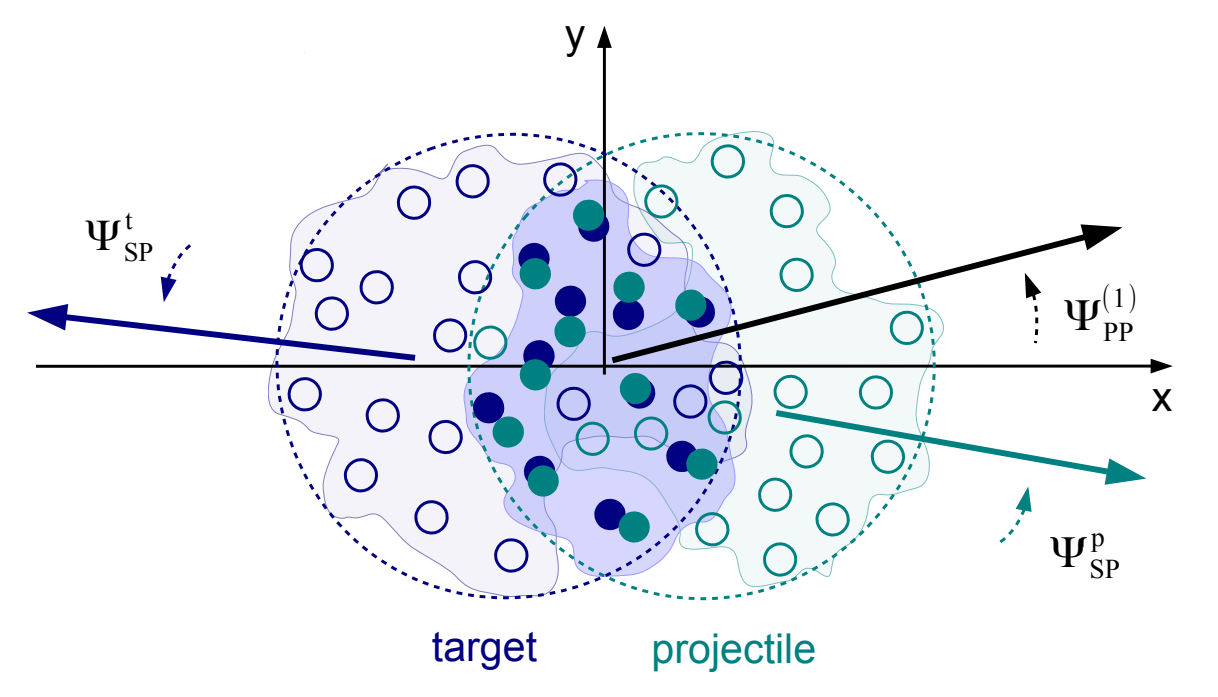
\includegraphics[width=0.75\linewidth]{images/v1_pp_sp.png}
\caption{Схематическое представление сталкивающихся ядера в плоскости перпендикулярной направлению пучка.}
\label{fig:pp_sp_rp}
\end{center}
\end{figure}
%

Таким образом, скорректированные на разрешение значения $v_1$ могут быть записаны следующим образом: 
%
\begin{equation}
    v_1 =  \frac{ \langle u_1 Q_1 \rangle }{R_1},
    \label{eq:v1_formula}
\end{equation}
%

\section{Влияние эффективности на измеренный $v_1$}

Коллективная анизотропия рожденных в столкновении частиц обычно измеряется дифференциально как функция центральности, поперечного и быстроты.
Неоднородная эффективность детектора в зависимости от этих переменных может приводить к неправильным значениям потоков при усреднении по этим переменным:
К примеру, при интегрировании по поперечному импульсу в границах $p_T^{1,2}$, при наличии неоднородной эффективности по поперечному импульсу $e(p_T)$ не будет совпадать с реальным значением потока:
%
\begin{equation}
    v_1( p_T^{1}, p_T^{2} ) \ne \int_{p_T^1}^{p_T^2} e(p_T) v_1(p_T) dp_T 
    \label{eq:v1_formula}
\end{equation}
Для коррекции на этот эффект, обычно функция $e(p_T, y)$ вычисляется из реалистичного Монте-Карло моделирования детектора и значения потока расчитываются с весом, обратным этой эффективности:
%
\begin{equation}
    v_1 = \frac{\int dp_T \int dy v_1(p_T, y) \frac{1}{e(p_T, y)} }{\int dp_T \int dy \frac{1}{e(p_T, y)} } 
    \label{eq:v1_formula}
\end{equation}

\section{Метод случайных подсобытий}

Для вычисления $R_1$ в эксперименте, можно воспользоваться попарными корреляциями $Q_1$-векторов (преобразование выполнено аналогично уравнению (\ref{eq:uq_transformation})): 
%
\begin{equation}
    \langle Q_1^a Q_1^b \rangle = V_a V_b \langle \cos(\Psi_a - \Psi_R) \cos(\Psi_b - \Psi_R) \rangle,
\end{equation}
%
где индексами $a$ и $b$ обозначены две различных группы частиц, в каждой из которых $Q_1$-вектор вычислялся независимо.

Наиболее простым методом вычисления разрешения является метод двух подсобытий:
%
\begin{equation}
    R_1\{a,b\} = \sqrt{ \langle Q_1^a Q_1^b \rangle } = \sqrt{ V_1^2 \langle \cos^{2}( \Psi_{a,b} - \Psi_R ) \rangle },
\end{equation}
где индексами $a$ и $b$ обозначены две группы частиц, идентичные по множественности и значению $v_1$, в которых $Q_1$-вектор вычислялся независимо.
В коллайдерных экспериментах, в качестве подсобытий $a$ и $b$ могут быть выбраны частицы в диапазонах по быстроте, симметрично относительно нуля.
В экспериментах с фиксированной мишенью, где такое выполнить невозможно, иногда пользуются методом, называемым метод случайных подсобытий.
Подсобытия $a$ и $b$ набираются случайным образом из частиц в данном кинематическом окне.
Этот метод прост в исполнении, однако корреляция $Q_1$-векторов из одной кинематической области может быть подвержена довольно большому вкладу непотоковых корреляций.

\section{Метод трех подсобытий}

Комбинируя различные попарные корреляции векторов, можно вычислить разрешение плоскости симметрии для данного $Q_1$-вектора:
%
\begin{equation}
    R_1\{a(b,c)\}  =  \sqrt { \frac{ \langle Q_1^a Q_1^b \rangle \langle Q_1^a Q_1^c \rangle }{ \langle Q_1^b Q_1^c \rangle} },
\end{equation}
%
где $a$, $b$ и $c$ --- три различных группы частиц, в каждой из которых $Q_1$-вектор вычислялся независимо.
Этот метод вычисления $R_1$ носит название метод трёх подсобытий.
Метод трёх подсобытий не накладывает ограничений на множественность частиц в каждой группе, что даёт большую свободу в выборе кинематических диапазонов для определения $Q_1$. 
Сравнивая $R_1$, вычисленный с использованием различных комбинаций $Q_1$ (к примеру $R_1\{a(b,c)\}$ и $R_1\{a(b,d)\}$) можно оценить вклад корреляций не связанных с коллективным движением частиц в полученный $R_1$ (непотоковые корреляции).
Сравнивая $v_1$ полученный относительно различных плоскостей симметрии (к примеру, $v_1\{a\}$ и $v_1\{b\}$), можно вычислить вклад непотоковых корреляций в результаты для направленного потока. 

\section{Корреляции не связанные с коллективным движением частиц}

Основными источниками непотоковых корреляций могут вызваны физическими эффектами: распады частиц, фемтоскопические корреляции (HBT), корреляции из-за закона сохранения поперечного (полного) импульса.
Также, непотоковые корреляции могут быть вызваны особенностями эксперимента: алгоритмы трекинга (слияние или разделение треков), особенности детекторов (поперечное распространение ливней в чувствительном объеме детектора). 
Непотоковые корреляции могут вносить значительную систематическую ошибку в измеренные значения $v_1$.
Основные методы учета вклада непотоковых корреляций включают использование частиц, имеющих значительное разделение по быстроте или поперечному импульсу и использование многочастичных корреляций.
Непотоковые корреляции могут присутствовать как между парами $Q_1$ векторов, так и между $u_1$ и $Q_1$ векторами.
Сравнивая значения потоков, полученных относительно различных плоскостей симметрии позволяет выявить наличие непотоковых корреляций в $\langle u_1 Q_1 \rangle$.

\section{Влияние азимутальной неоднородности аксептанса детектора}

Значительный вклад в результаты измерения азимутальных потоков может вносить неоднородность аксептанса детектора. 
Азимутальная анизотропия аксептанса искажает распределение $u_1$ $Q_1$-векторов, которые в идеальном случае должны быть равномерными. 
Для коррекции этого эффекта был использован метод, описаный в работе~\cite{Selyuzhenkov:2007zi}.
Поскольку плоскость реакции распределена равномерно, в пределах большого количества столкновений формулу~(\ref{eq:v1_formula}) можно преобразовать следующим образом:
%
\begin{equation}
    v_1 =  2\frac{ \langle x_1 X_1 \rangle }{R_1^X} = 2\frac{ \langle y_1 Y_1 \rangle }{R_1^Y},
    \label{eq:v1_formula}
\end{equation}
%
где $x_1$ и $y_1$ --- компоненты $u_1$-вектора, $X_1$ и $Y_1$ --- компоненты $Q_1$-вектора и $R_1^{X,Y}$ --- разрешение плоскости симметрии, вычисленное при помощи корреляций компонент $Q_1$-векторов.
Азимутальная неоднородность детектора нарушает это равенство.

Основные эффекты, вызываемые неоднородностью аксептанса могут быть выражены в следующем:
\begin{enumerate}
    \item Сдвиг $u_1$ ($Q_1$) вектора из-за ненулевых средних значений компонент:
    \begin{equation}
        \langle x_1 \rangle \ne 0, \langle y_1 \rangle \ne 0
    \end{equation}
    Коррекция на этот эффект носит название перецентровки.
    \item Поворот $u_1$ ($Q_1$) векторов. Коррекция на этот эффект называется коррекцией поворота
    \item Сужение/Расширение распределения компонент $u_1$ ($Q_1$) вектора. Коррекция носит название ремасштабирования.
\end{enumerate}

После применения описанных выше коррекций, распределение $u_1$ ($Q_1$) вектора становится равномерным по азимутальному углу.
Систематический вклад остаточной азимутальной неоднородности аксептанса детектора может быть оценен сравнением результатов полученных с использованием различных компонент $u_1$ и $Q_1$-векторов. 

\section{Вычисление $Q_1$ при помощи модульных детекторов}

В данной работе для восстановления плоскости симметрии используются фрагменты ядра, которые взаимодействовали с областью перекрытия лишь упруго (спектаторы). 
Спектаторные фрагменты отталкиваются областью перекрытия в плоскости реакции (см.~\ref{fig:pp_sp_rp}), поэтому могут быть использованы для реконструкции плоскости симметрии. 
Часто в экспериментах по столкновению тяжёлых ионов регистрация спектаторных частиц выполняется при помощи детекторов, имеющих модульную структуру. 
В таком случае $Q_1$-вектор будет определяться суммарной азимутальной анизотропией распределения сигнала по модулям:
%
\begin{equation}
    Q_1  = \frac{1}{C} \sum_{k=1}^M w_k ( \cos \varphi, \sin \varphi ),
\end{equation}
%
где $k$ --- индекс модуля, $M$ --- число модулей, использованных в построении $Q_1$-вектора, $w_k$ --- сигнал в данном модуле, $\varphi$ --- азимутальный угол данного модуля. 
Нормировочный коэффициент $C$ может также принимать значения $C=|Q_1|$ (метод плоскости события) или $C=\sum_{k=1}^M w_k$ (метод скалярного произведения).
Взвешивание на сигнал в данном модуле необходимо, поскольку в один и тот же модуль могут попасть более одной частицы.
Корреляции между $Q_1$-векторами, определёнными из разных групп модулей одного детектора также могут быть подвержены непотоковым корреляциям.
К примеру, между соседними модулями может происходить перетекание сигнала вследствие конструкционных особенностей детектора (например, в адронных калориметрах присутствует поперечное распространение ливней).
Также при распаде осколков сталкивающихся ядер, фрагменты могут вызвать отклик соседних модулей, что снова приведёт к корреляциям между модулями, которые не относятся к коллективному движению частиц.
Такие корреляции могут искажать значения разрешения.
Для учёта этих эффектов можно определить $Q_1$-вектора из треков рожденных частиц с достаточным разделением по быстроте между тракеториями и модулями.

\section{Выводы к главе 1}

В главе были описаны основные механизмы образования коллективной анизотропии и представлены обоснования необходимости ее измерения.
Было представлено введение в теорию измерения анизотропных потоков. 
В главе приведены методы вычисления $v_1$ и коррекции результатов на флуктуации плоскости симметрии вокруг плоскости реакции.
Описаны методы вычисления поправочного коэффициента разрешения, такие как метод случайных подсобытий и метод трёх подсобытий.
Представлены основные эффекты, не связанные с коллективным движением частиц и их влияние на полученные значения $v_1$.
В главе описано влияние азимутальной неоднородности детектора на результаты измерения коллективных эффектов и приведены коррекции направленные на подавление этих эффектов.
В главе обсуждается способ коррекции на неоднородную эффективность установки и методы вычисления $Q_1$ при помощи модульных детекторов.    